\chapter{Conditional Distribution based on Quantile Regression for Time Series}

In the previous section, we presented two methods for estimating a single $\alpha$-quantile by using QR. However, to build a CDF from an array of quantile, we propose to jointly estimate them, in order to explore the connection across different quantiles. 

Let the finite discretization of the interval $[0,1]$ be composed of a sequence of probabilities $0 < \alpha_1 < \alpha_2 < \dots < \alpha_{|J|} < 1$ and denote as $A$ the set $A = \{ \alpha_j \mid j \in J \}$, where $J$ is an index set for the probabilities $\alpha$. 
The $\alpha$-quantiles are, from this point forward, indexed by $j$, to account for the different models that are simultaneously estimated. A property that must be respected is the monotonicity of the Quantile function $Q$, such that $q_{\alpha_1} \leq q_{\alpha_2} \dots \leq q_{\alpha_{|J|}}$.
The sequence of quantiles define a continuous quantile function after interpolation, and finally a CDF after inverting the estimated quantile function.

The following sections present how to jointly estimate quantiles through QR for each one of the two methods.
% To estimate the conditional distribution, $\hat{Q}_{Y_{t+h}|X_{t+h},Y_t, Y_{t-1}, \dots} (\alpha,\cdot)$, of time series $\{y_t\}_{t \in T}$ $h$-steps ahead, where $X_{t+h}$ makes reference to a vector of exogenous variables. Once the conditional distribution is estimated, future scenarios can be obtained by simulation. %In this paper, we focus on the 1-step ahead forecasting ($h=1$) and the model don't include any covariates but its own autoregressive terms. 



\section{Linear Model}

As we are interested on the conditional distribution as a whole, we estimate multiple quantiles at once. In order to produce a coherent distribution function, the output of the problem must respect certain properties, such as being monotone increasing. 
Besides that, one can expect that the value of similar quantiles be produced by similar models. If the coefficient of a given $p$ covariate changes too abruptly with respect to a change on the probability $\alpha$, there is a high probability that the estimation did not produce good results rather than this noise belonging to the true model.  In order to correct this much common behavior in QR estimation, we introduce a second derivative filter,given by the discrete approximation shown below:
\begin{equation}
D_{\alpha_j}^{2} \beta_{pj} := \frac{\left(\frac{\beta_{p,j+1}-\beta_{pj}}{\alpha_{j+1}-\alpha_{j}}\right)-\left(\frac{\beta_{p,j}-\beta_{p,j-1}}{\alpha_{j}-\alpha_{j-1}}\right)}{\alpha_{j+1}-\alpha_{j-1}}. 
\end{equation}
With this approach, one can keep track on the crossing quantiles issue as well as using a interquartile structure as a strategy to reduce noise on estimation %! explicar melhor o porquê
The works by \cite{zou_regularized_2008, jiang_interquantile_2014} also use multiple quantile regressions at once and make use of interquantile similarities to produce regularization on the quantiles. In \cite{zou_regularized_2008}, the author uses the norm $\| \beta \|_{1\infty}=\sum_{p=1}^{|P|} \max\{ |\beta_j^{(k)} |\}$ as penalization. Such penalization is imposed on the maximum value among all quantiles for a given covariate. This idea is extended by \cite{jiang_interquantile_2014}, that uses a fused AdaLASSO mixing the LASSO penalization with the absolute interquantile difference.

The statistical model \textbf{Quantile Regularized Adaptive LASSO (QRAL)} is defined by the vector of coefficients $\beta_{0}$ and the matrix of size $|P| \times |J|$ of regressor coefficients $\beta_{pj}$. These coefficients are the solution from the minimization problem given below:
% \begin{IEEEeqnarray}{lr}  % para duas colunas
% 	\underset{\beta_{0j},\beta_j}{\text{min}} \sum_{j \in J} \left( \sum_{t\in T}\rho_{\alpha_j}(y_{t}-(\beta_{0j} + \beta_j^T x_t)) \right.  \span \nonumber \\
% 	\span \left. + \lambda\  \sum_{p \in P} w_{pj}^\delta \mid  \beta_{pj} \mid \right) + \gamma \sum_{p \in P} \sum_{j \in J'} |D^2_{pj}|,\label{eq:adalasso_model}
% \end{IEEEeqnarray}
\begin{align} % para uma coluna
&	\underset{\beta_{0j},\beta_j}{\text{min}} \sum_{j \in J} \left( \sum_{t\in T}\rho_{\alpha_j}(y_{t}-(\beta_{0j} + \beta_j^T x_t)) \right.   \left. + \lambda\  \sum_{p \in P} w_{pj}^\delta \mid  \beta_{pj} \mid \right) + \gamma \sum_{p \in P} \sum_{j \in J'} |D^2_{\alpha_j}\beta_{pj}|, \span \label{eq:adalasso_model_mat1}\\
 & \text{subject to} & \nonumber \\
	&\beta_{0j} + \beta_{j}^T x_{t} \leq \beta_{0,j+1} + \beta_{j+1}^T x_{t}, & \forall t \in T, \forall j \in J_{(-1)},\label{eq:adalasso_model_mat2}
\end{align}
where the weights $w_{pj} = 1/\tilde{\beta}_{pj}$ and $\tilde \beta_{pj}$ are the coefficients from the first-step LASSO estimation. The parameter $\delta$ is an exponential parameter usually set to 1.
The sum of absolute values that compose the second derivative filter $\sum_{j \in J'}\sum_{p \in P}|D_{\alpha_j}^{2}\beta_{pj}|$ is added on the objective function multiplied by a tuning parameter $\gamma$, where the set $J'=\{2,\dots,|J|-1 \}$.

\section{Nonparametric Quantile Regression}

%The quantile estimation is done for different values of $\lambda_2$. By using different levels of penalization on the second difference, the estimation can be more or less adaptive to the fluctuation. It is important to notice that the usage of the $\ell_1$-norm as penalty leads to a piecewise linear solution $q_{t \alpha}$. % Referenciar?

To jointly estimate multiple quantiles, the optimization problem that defines NQR is changed to the following:
\begin{align}
& \underset{q_{tj}}{\min} \sum_{j \in J} \left( \sum_{t\in T'} \rho_{\alpha_j} \left( y - q_{tj} \right)  +\lambda_1  \sum_{t\in T'}|D_{x_t}^{1}q_{tj}| +\lambda_2  \sum_{t\in T'}|D_{x_t}^{2}q_{tj}| \right), \span \label{eq:nqr-mat1} \\
& q_{t j} \leq q_{t j+1}, &  \forall t \in T, \forall j \in J_{(-1)},\label{eq:nqr-mat2}
\end{align}
where equation (\ref{eq:nqr-mat2}) is a noncrossing constraint and $T'$ is the index set $T' = \{ 2, \dots, |T|-1 \}$.


Figure \ref{fig:npqar-results} shows, for realistic data, how the nonlinear estimator can have different degrees of fit on the data.
The procedure used to choose the tuning parameters $\lambda_1$ and $\lambda_2$ is a topic discussed in the next session, where the cross-validation methodology is presented. The importance of this choice is evident when seeing Figure \ref{fig:npqar-results}, as there is a big tradeoff between bias and variance.
% \begin{figure*}[htp]
%   \centering
%   \begin{minipage}[t]{0.4\linewidth}
%     \centering
%     \begin{minipage}[t]{\linewidth}
%       \centering     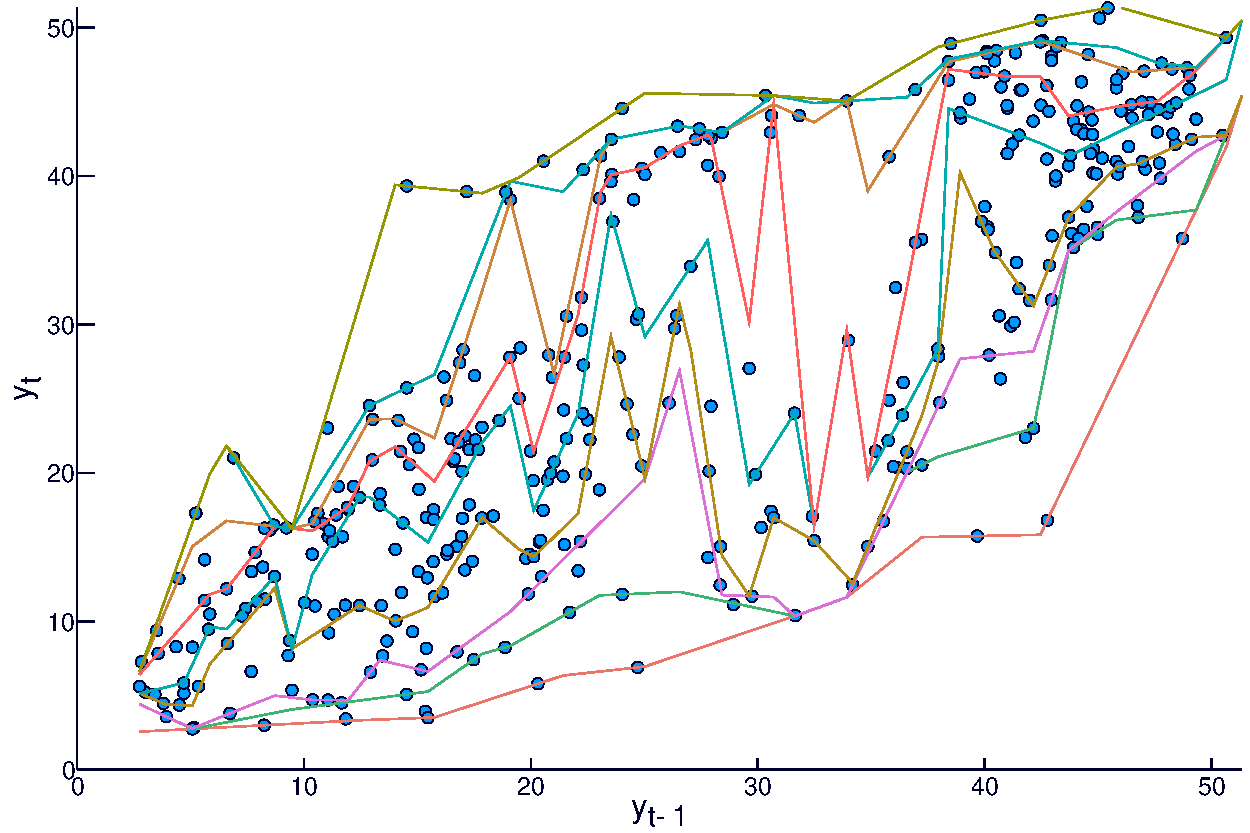
\includegraphics[width=\textwidth]{Images/icaraizinho-crossing-01}
% 	  \subcaption{$\lambda_1 = 0, \, \lambda_2 = 0.1$}
% 	  \label{fig:nonlinear1}
%     \end{minipage}
%     \begin{minipage}[b]{\linewidth}
%       \centering     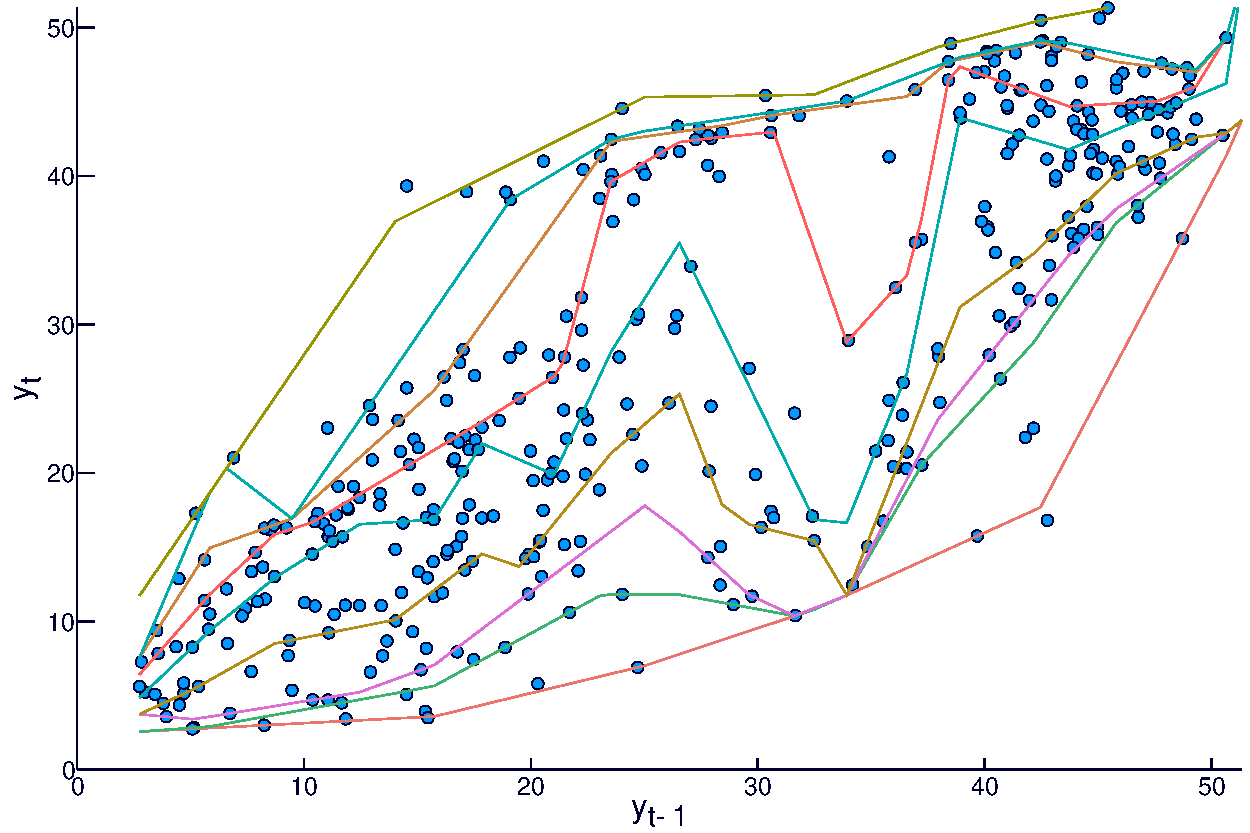
\includegraphics[width=\textwidth]{Images/icaraizinho-crossing-03}
%       \subcaption{$\lambda_1 = 0, \, \lambda_2 = 0.3$}
%     \end{minipage}
%      \begin{minipage}[b]{\linewidth}
%       \centering     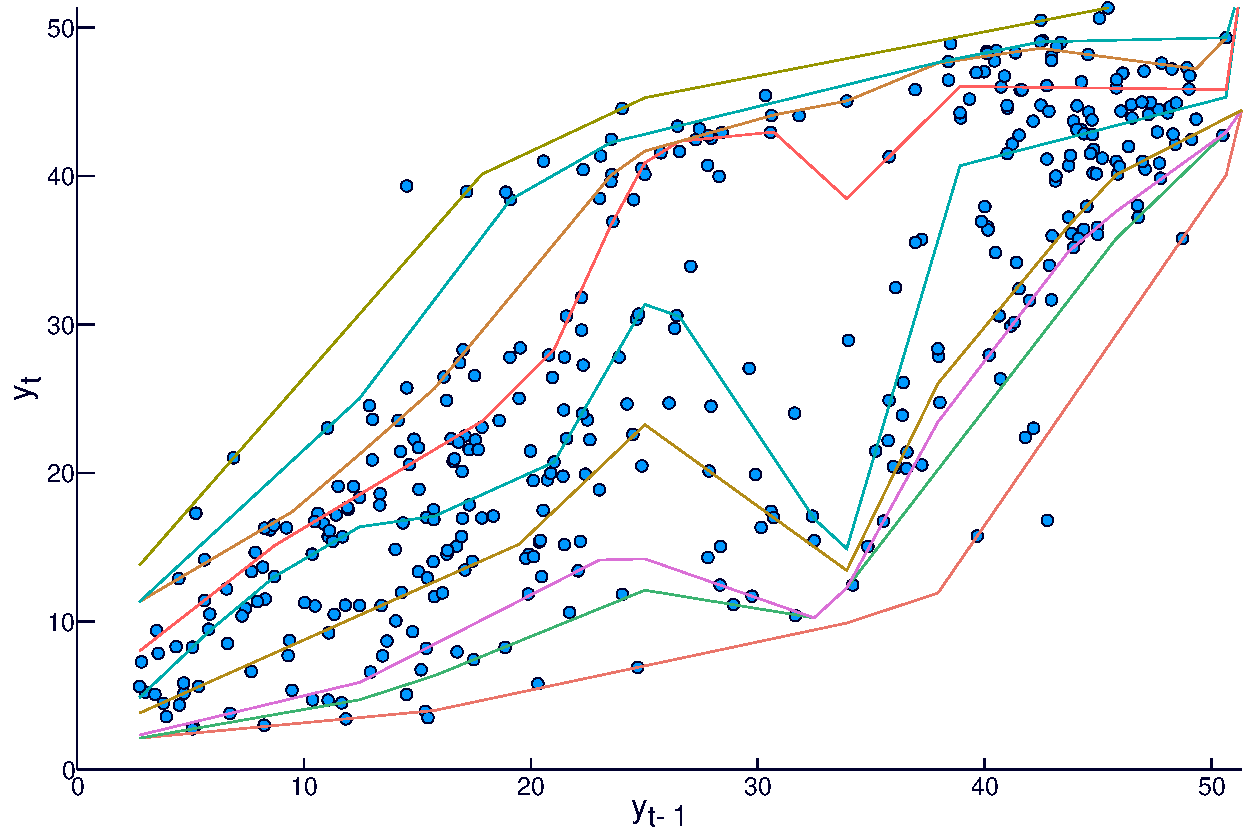
\includegraphics[width=\textwidth]{Images/icaraizinho-crossing-1}
%       \subcaption{$\lambda_1 = 0, \, \lambda_2 = 1$}
%      \end{minipage}
%   \end{minipage}
%   \begin{minipage}[t]{0.4\linewidth}
%     \centering
%     \begin{minipage}[t]{\linewidth}
%       \centering     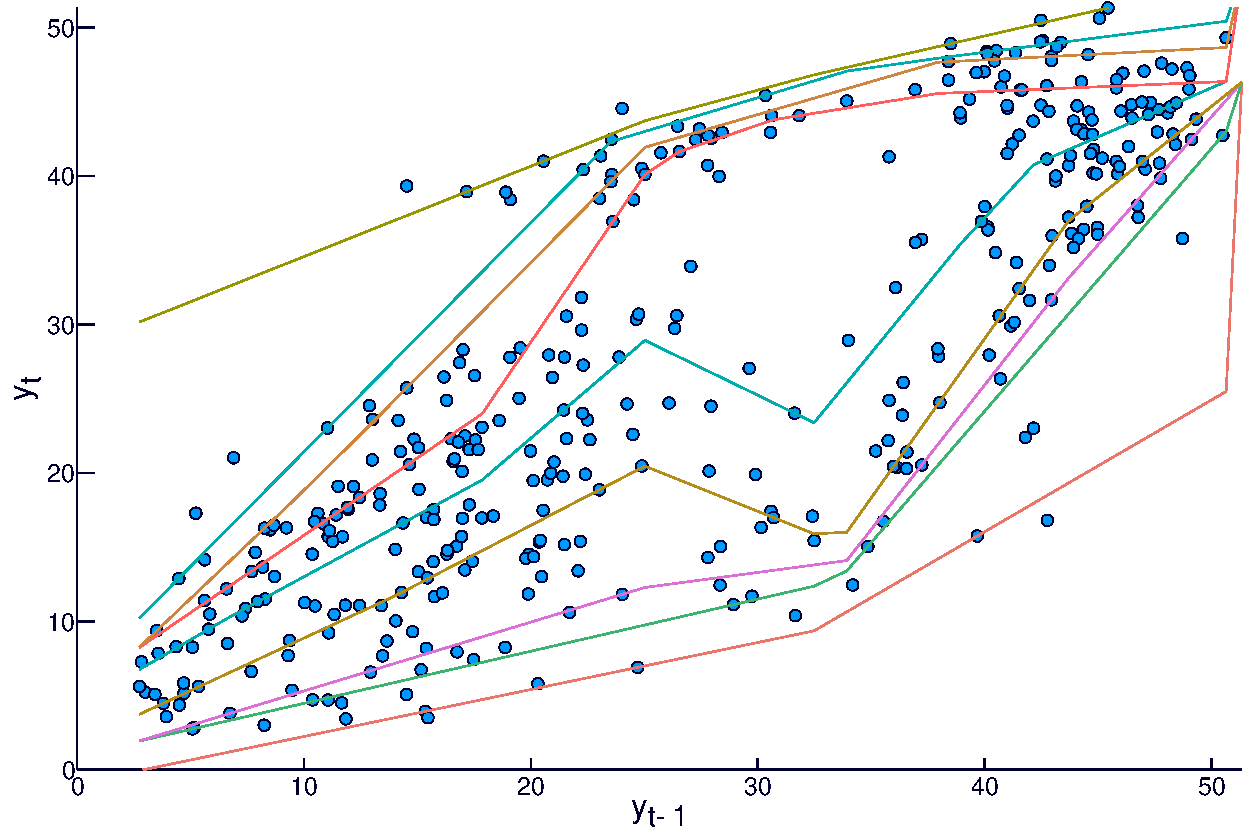
\includegraphics[width=\textwidth]{Images/icaraizinho-crossing-3}
%       \subcaption{$\lambda_1 = 0, \, \lambda_2 = 3$}
%     \end{minipage}
%     \begin{minipage}[b]{\linewidth}
%       \centering     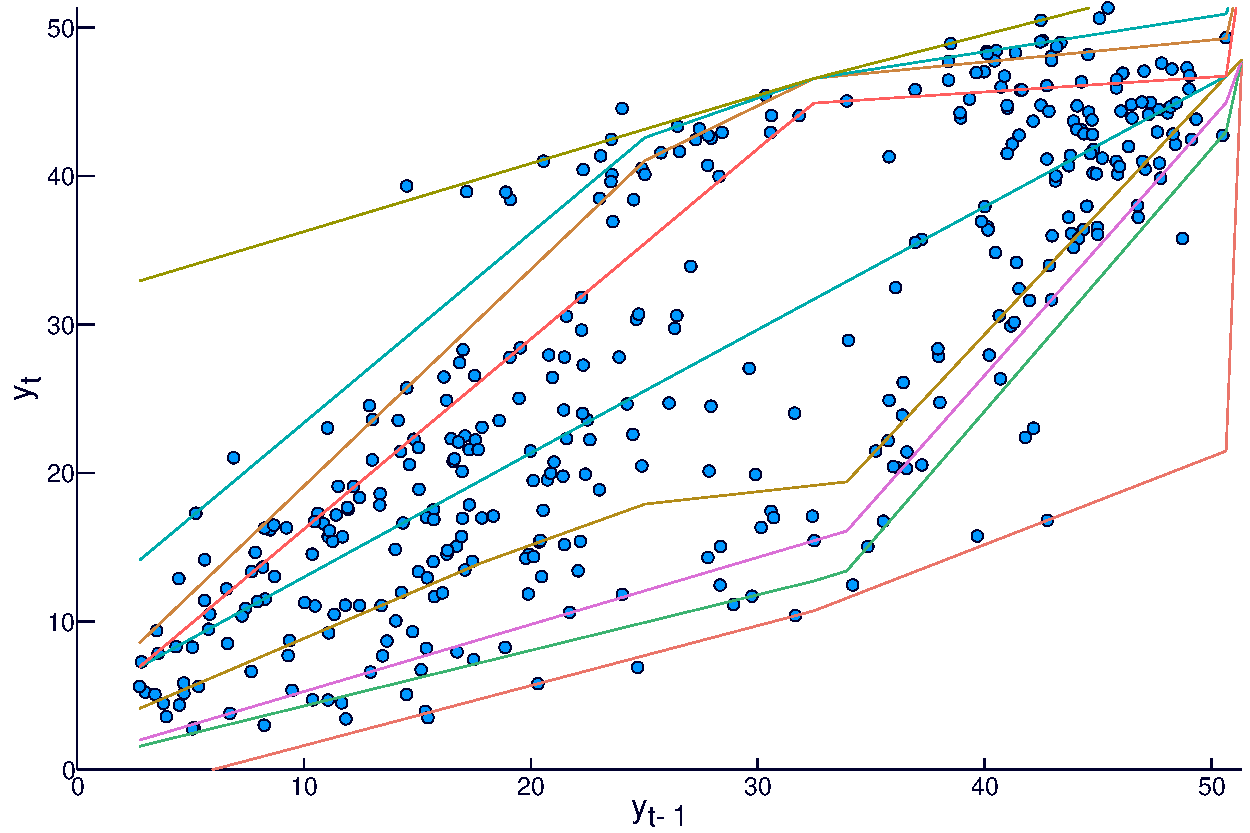
\includegraphics[width=\textwidth]{Images/icaraizinho-crossing-10}
%       \subcaption{$\lambda_1 = 0, \, \lambda_2 = 10$}
%     \end{minipage}
%      \begin{minipage}[b]{\linewidth}
%       \centering     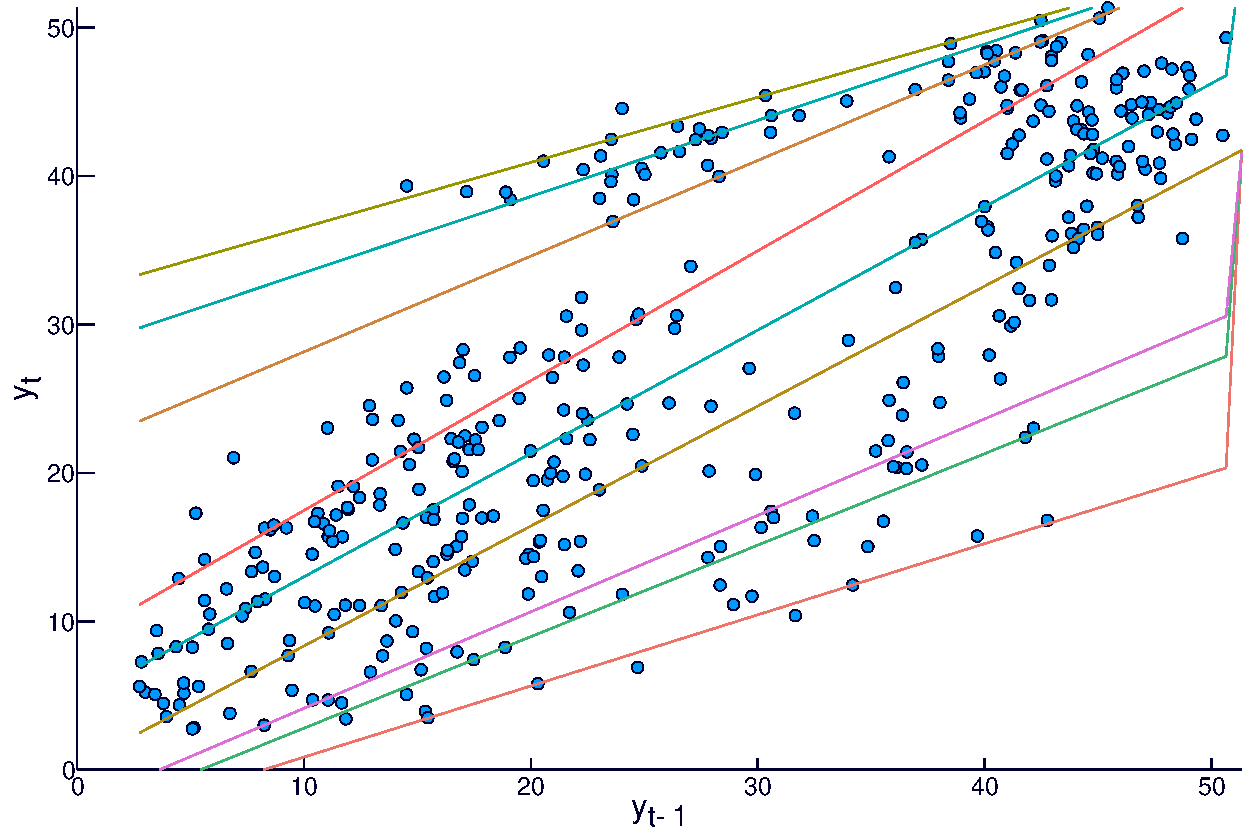
\includegraphics[width=\textwidth]{Images/icaraizinho-crossing-200}
%       \subcaption{$\lambda_1 = 0, \, \lambda_2 = 200$}
%       \label{fig:npqar-cross}
%      \end{minipage}
%   \end{minipage}
%   \caption{Quantile estimations for a few different values of $\lambda_2$. The quantiles represented here are $\alpha = (5\%, 10\%, 25\%, 50\%, 75\%, 90\%, 95\%)$. When $\lambda_2 = 0.1$, on the upper left, estimated quantiles clearly overfit the data. On the other extreme, when $\lambda_2=200$, the nonparametric estimator converges to the linear model.}
%   \label{fig:npqar-results}
% \end{figure*}

\begin{figure*}[htp]
  \centering
  \begin{minipage}[t]{0.4\linewidth}
    \centering
    \begin{minipage}[t]{\linewidth}
      \centering     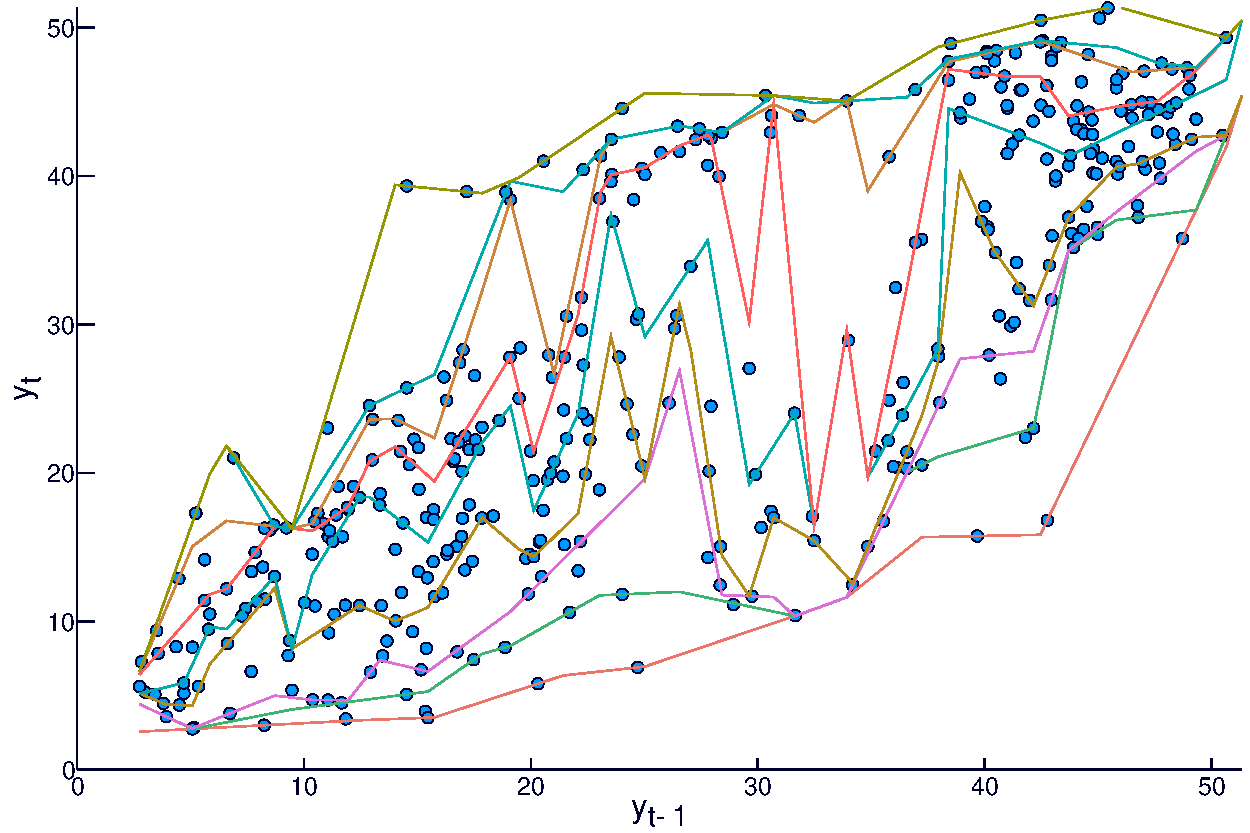
\includegraphics[width=\textwidth]{Images/icaraizinho-crossing-01}
	  {(a) $\lambda_1 = 0, \, \lambda_2 = 0.1$}
	  % \label{fig:nonlinear1}
    \end{minipage}
    \begin{minipage}[b]{\linewidth}
      \centering     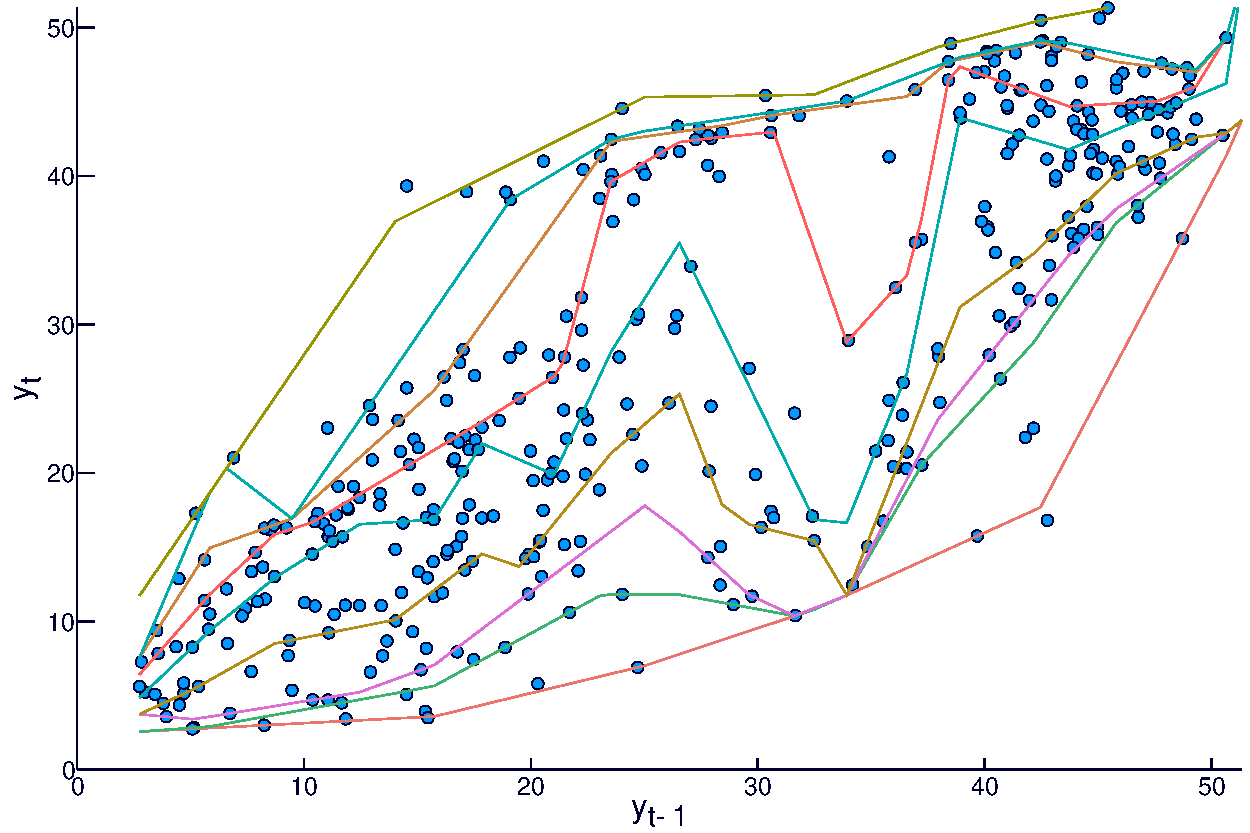
\includegraphics[width=\textwidth]{Images/icaraizinho-crossing-03}
      {(c) $\lambda_1 = 0, \, \lambda_2 = 0.3$}
    \end{minipage}
     \begin{minipage}[b]{\linewidth}
      \centering     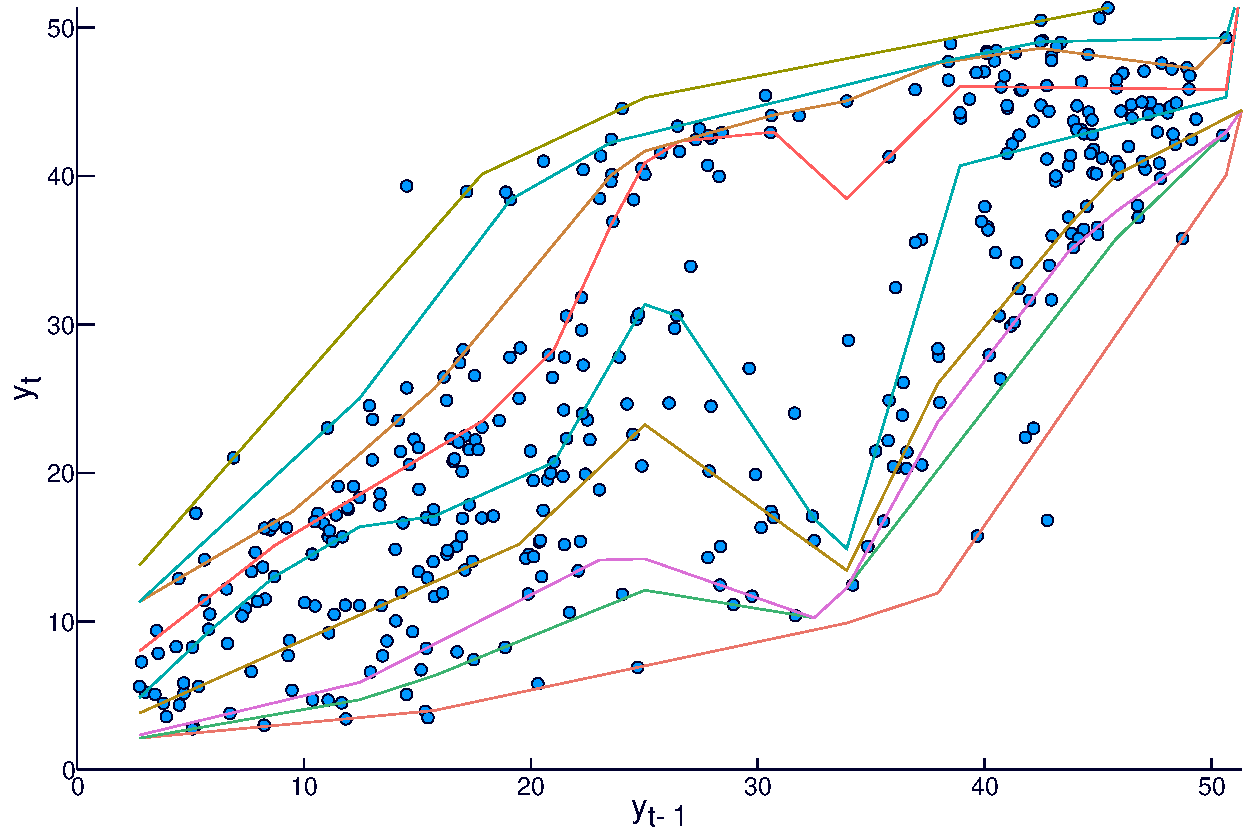
\includegraphics[width=\textwidth]{Images/icaraizinho-crossing-1}
      {(e) $\lambda_1 = 0, \, \lambda_2 = 1$}
     \end{minipage}
  \end{minipage}
  \begin{minipage}[t]{0.4\linewidth}
    \centering
    \begin{minipage}[t]{\linewidth}
      \centering     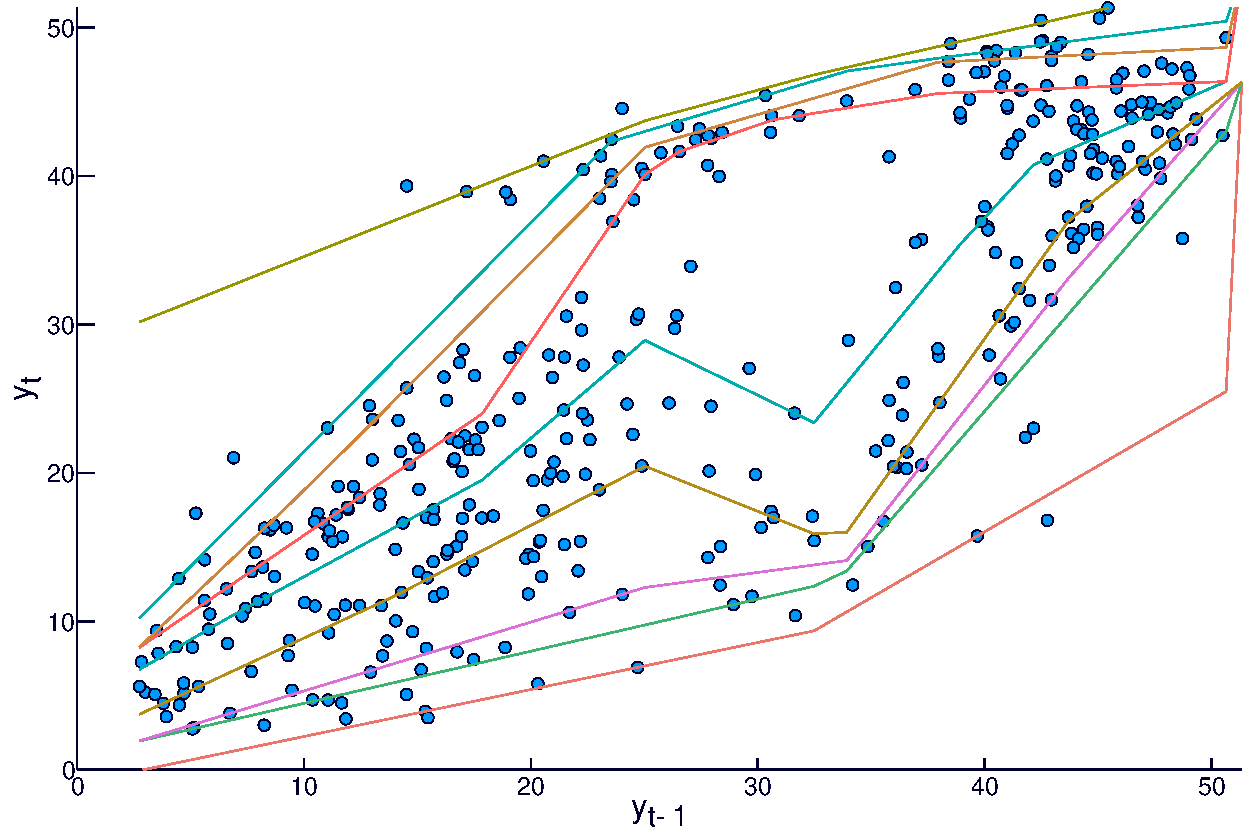
\includegraphics[width=\textwidth]{Images/icaraizinho-crossing-3}
      {(b) $\lambda_1 = 0, \, \lambda_2 = 3$}
    \end{minipage}
    \begin{minipage}[b]{\linewidth}
      \centering     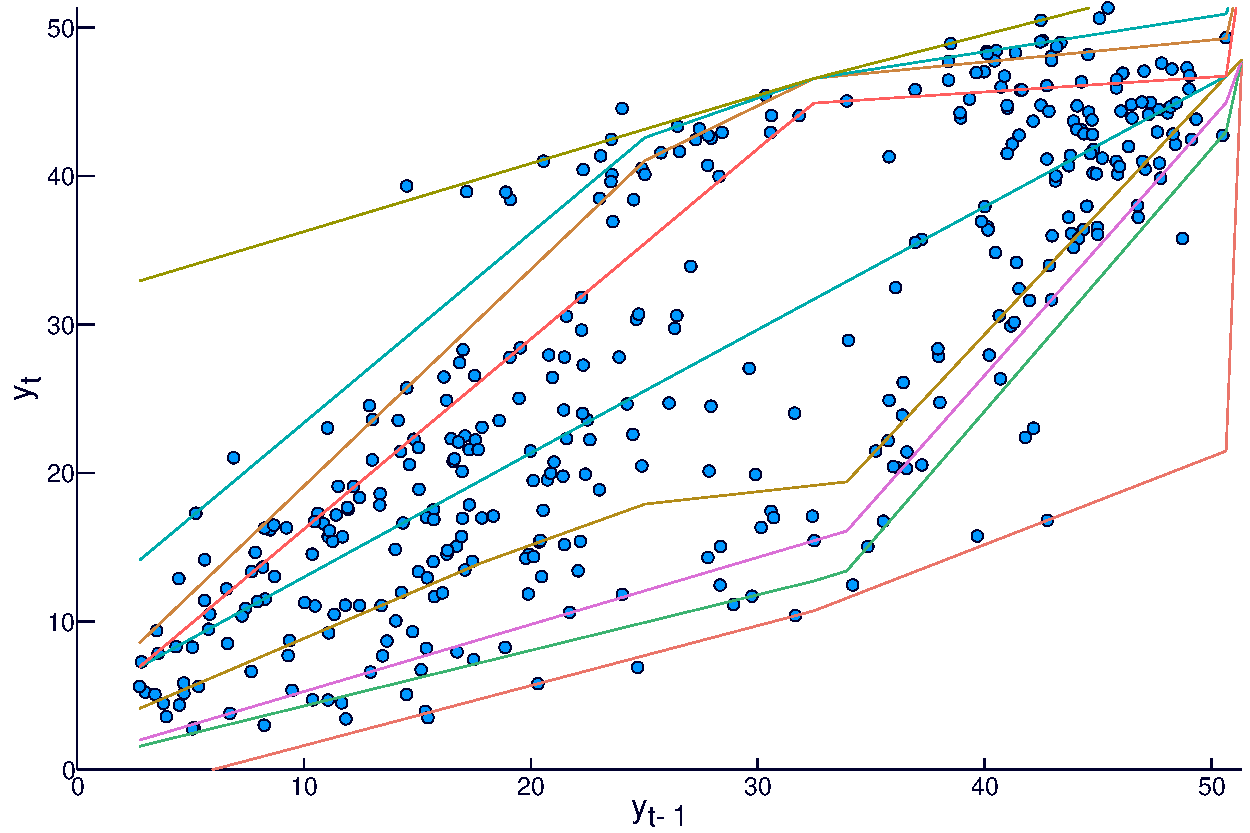
\includegraphics[width=\textwidth]{Images/icaraizinho-crossing-10}
      {(d) $\lambda_1 = 0, \, \lambda_2 = 10$}
    \end{minipage}
     \begin{minipage}[b]{\linewidth}
      \centering     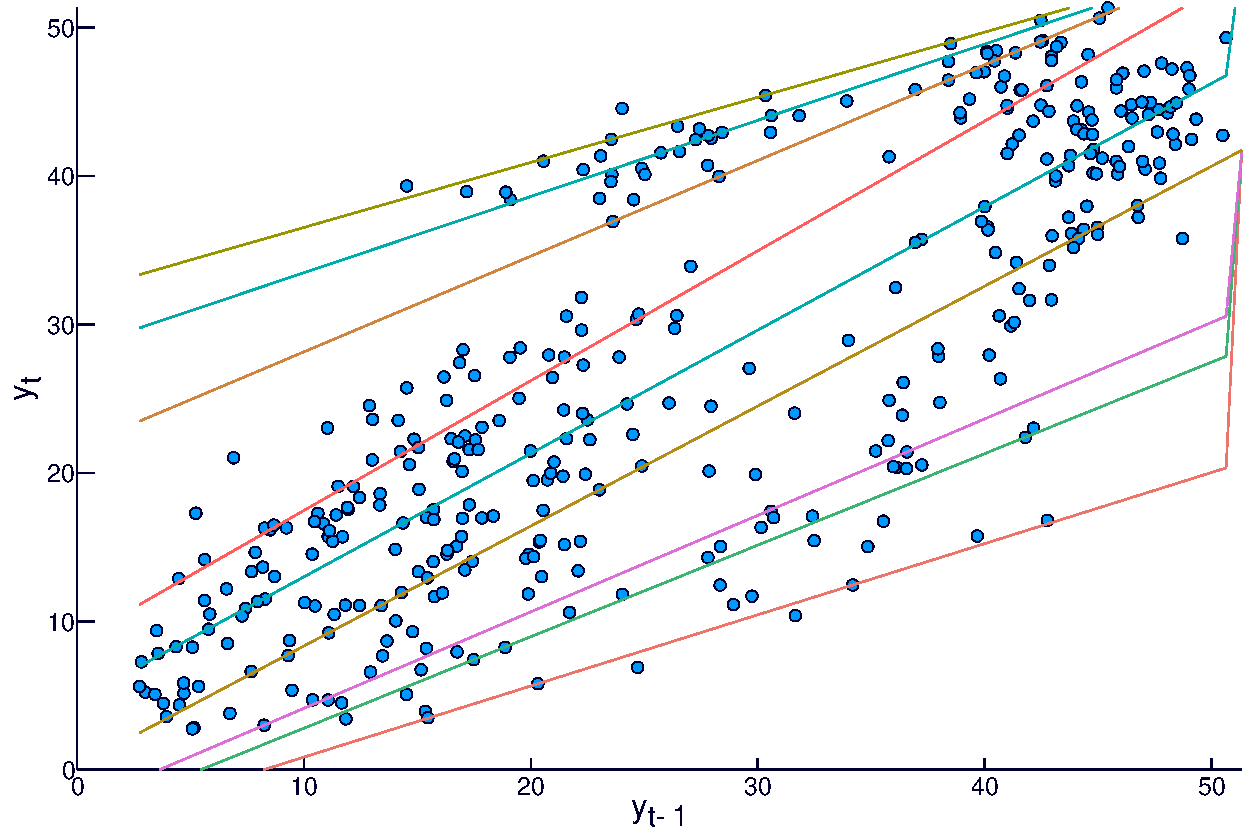
\includegraphics[width=\textwidth]{Images/icaraizinho-crossing-200}
      {(f) $\lambda_1 = 0, \, \lambda_2 = 200$}
      \label{fig:npqar-cross}
     \end{minipage}
  \end{minipage}
  \caption{Quantile estimations for a few different values of $\lambda_2$. The quantiles represented here are $\alpha = (5\%, 10\%, 25\%, 50\%, 75\%, 90\%, 95\%)$. When $\lambda_2 = 0.1$, on the upper left, estimated quantiles clearly overfit the data. On the other extreme, when $\lambda_2=200$, the nonparametric estimator converges to the linear model.}
  \label{fig:npqar-results}
\end{figure*}

